\documentclass[10pt]{article}

\usepackage{hyperref}
\usepackage{enumerate}
\usepackage{amsmath}
\usepackage{graphicx}
%% --------------------------------------------------------------
\title{A very simple Latex}
\author{Tiep Vu, Penn State}
\date{July 2016}
%% --------------------------------------------------------------
\begin{document}
\maketitle
\section{Problem} % (fold)
\label{sec:problem}
Given three real numbers $a, b, c$, solve the equation: 
\begin{equation}
	\label{eqn:problem}
    ax^2 + bx + c = 0
\end{equation}
% section problem (end)
\section{Solution} % (fold)
\label{sec:solution}
\begin{enumerate}
	\item $a = 0$
		\begin{itemize}
			\item $b = 0, c \neq 0 \Rightarrow$ there is no solution for equation (\ref{eqn:problem}).

			\item $b \neq 0 $
			\item ...
		\end{itemize}

	\item $a \neq 0$. Let $\Delta = b^2 - 4ac.$ ...
\end{enumerate}
% section solution (end)

\section{Example} % (fold)
\label{sec:example}
Solve equation: $x^2 - x - 2 = 0$. \\
Looking at Figure \ref{fig:example1}, the solution is $x \in \{-1, 2\}$
\begin{figure}[h]
\label{fig:example1}
\centering	
	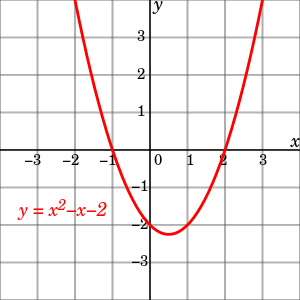
\includegraphics[scale = 0.4]{figs/fig1.png}
	\caption{The caption is here}
\end{figure}
% section example (end)

\section{More example} % (fold)
\label{sec:more_example}
\begin{table}[]
\centering
\caption{My caption}
\label{my-label}
\begin{tabular}{|l|l|l|l|l|}
\hline
$a$ & $b$  & $c$ & $x_1$ & $x_2$ \\ \hline
1 & -4 & 3 & 1    & 3    \\ \hline
1 & -2 & 1 & 1    & 1    \\ \hline
\end{tabular}
\end{table}
% section more_example (end)

\section{Citations} % (fold)
\label{sec:citations}
Tiep Vu \textit{et. al.} \cite{vu2015dfdl}
% section citations (end)

\bibliographystyle{IEEEtran}
\bibliography{refs}
\end{document}